% fig_6_g_hypothesis_validation.tex
% Traffic-light hypothesis validation summary
% Compile: pdflatex fig_6_g_hypothesis_validation.tex
\documentclass[tikz,border=5pt]{standalone}

\usepackage[T1]{fontenc}
\usepackage[utf8]{inputenc}
\usepackage{amsmath,amssymb}
\usepackage{tikz}
\usetikzlibrary{arrows.meta, positioning, shapes.geometric, calc}

% ── Color palette ──────────────────────────────────────────────────
\definecolor{greenLight}{HTML}{4CAF50}
\definecolor{greenLightFill}{HTML}{E8F5E9}
\definecolor{yellowLight}{HTML}{FFC107}
\definecolor{yellowLightFill}{HTML}{FFF8E1}
\definecolor{headerBg}{HTML}{263238}
\definecolor{headerText}{HTML}{ECEFF1}
\definecolor{rowEven}{HTML}{FAFAFA}
\definecolor{rowOdd}{HTML}{F5F5F5}
\definecolor{borderGray}{HTML}{B0BEC5}
\definecolor{textDark}{HTML}{212121}
\definecolor{evidenceBlue}{HTML}{1565C0}

\begin{document}
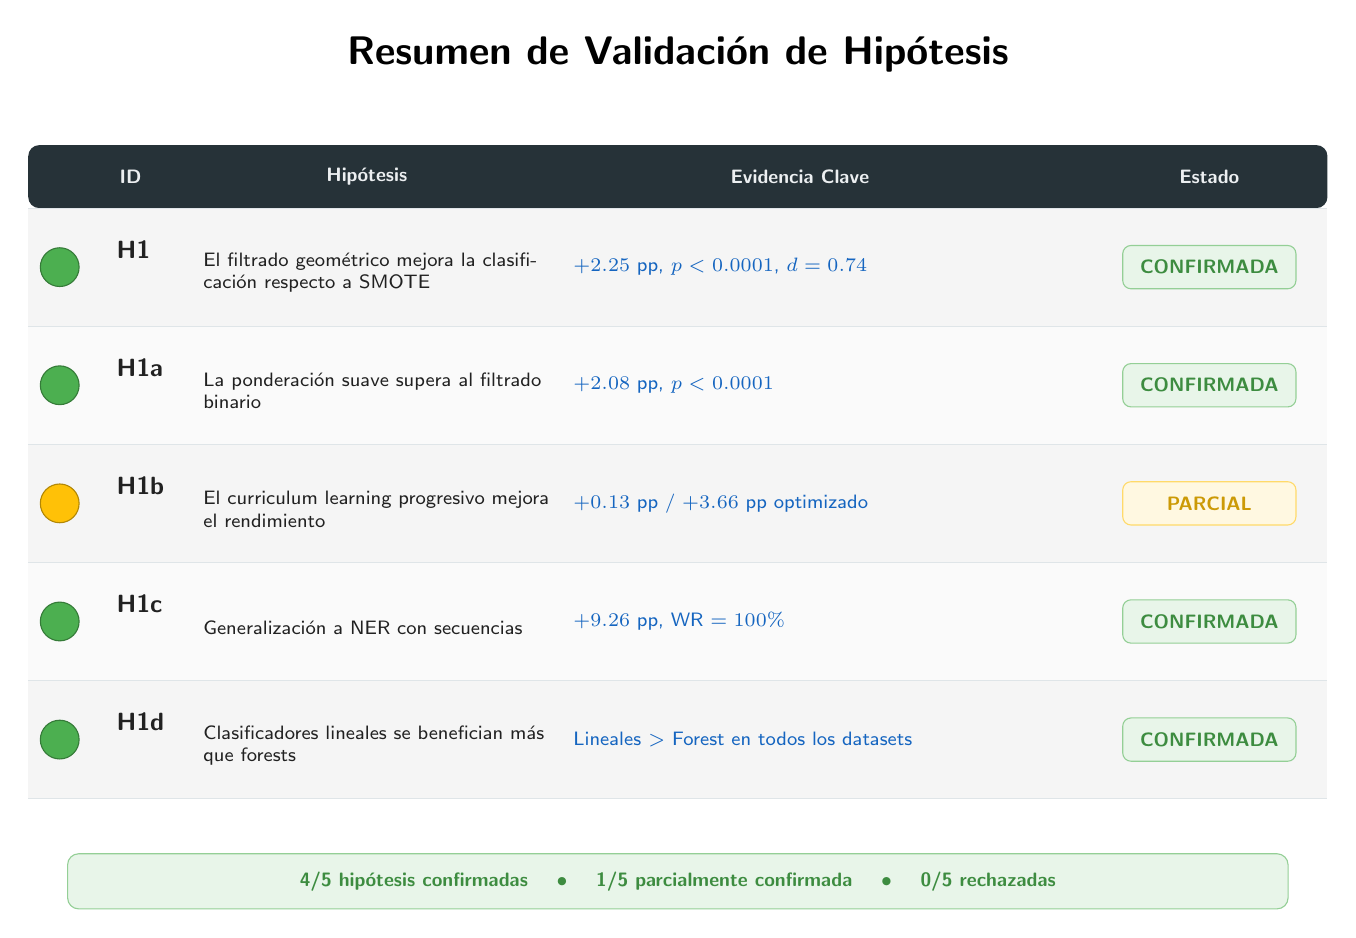
\begin{tikzpicture}[
    % ── shared styles ───────────────────────────────────────────────
    traffic green/.style={
        circle, fill=greenLight, draw=greenLight!70!black,
        inner sep=0pt, minimum size=14pt,
        font=\tiny\bfseries, text=white,
    },
    traffic yellow/.style={
        circle, fill=yellowLight, draw=yellowLight!70!black,
        inner sep=0pt, minimum size=14pt,
        font=\tiny\bfseries, text=white,
    },
    status confirmed/.style={
        rectangle, rounded corners=3pt,
        fill=greenLightFill, draw=greenLight!60,
        font=\sffamily\scriptsize\bfseries, text=greenLight!80!black,
        minimum height=0.55cm, minimum width=2.2cm,
        align=center,
    },
    status partial/.style={
        rectangle, rounded corners=3pt,
        fill=yellowLightFill, draw=yellowLight!60,
        font=\sffamily\scriptsize\bfseries, text=yellowLight!80!black,
        minimum height=0.55cm, minimum width=2.2cm,
        align=center,
    },
]

% =============================================================
%  Layout constants
% =============================================================
\def\rowH{1.5}    % row height
\def\tableW{16.5} % total table width
\def\colLight{0.8}   % traffic light column width
\def\colID{1.0}      % hypothesis ID column
\def\colDesc{5.5}    % description column
\def\colEvid{6.5}    % evidence column
\def\colStatus{2.7}  % status column

% =============================================================
%  Title
% =============================================================
\node[font=\sffamily\Large\bfseries, anchor=south] at (0.5*\tableW, 0.8)
    {Resumen de Validaci\'{o}n de Hip\'{o}tesis};

% =============================================================
%  Header row
% =============================================================
\fill[headerBg, rounded corners=4pt]
    (0, 0) rectangle (\tableW, -0.8);

\def\xLight{0.4}
\def\xID{1.3}
\def\xDesc{4.3}
\def\xEvid{9.8}
\def\xStatus{15.0}

\node[font=\sffamily\scriptsize\bfseries, text=headerText] at (\xLight, -0.4) {};
\node[font=\sffamily\scriptsize\bfseries, text=headerText] at (\xID, -0.4) {ID};
\node[font=\sffamily\scriptsize\bfseries, text=headerText] at (\xDesc, -0.4) {Hip\'{o}tesis};
\node[font=\sffamily\scriptsize\bfseries, text=headerText] at (\xEvid, -0.4) {Evidencia Clave};
\node[font=\sffamily\scriptsize\bfseries, text=headerText] at (\xStatus, -0.4) {Estado};

% =============================================================
%  ROW 1: H1 - CONFIRMADA (green)
% =============================================================
\def\ry{-0.8}
\fill[rowOdd] (0, \ry) rectangle (\tableW, \ry-\rowH);
\draw[borderGray!40] (0, \ry) -- (\tableW, \ry);

\node[traffic green] at (\xLight, \ry-0.5*\rowH) {};

\node[font=\sffamily\small\bfseries, text=textDark, anchor=west]
    at (\xID-0.3, \ry-0.35*\rowH) {H1};
\node[font=\sffamily\scriptsize, text=textDark, anchor=west, text width=4.5cm]
    at (\xDesc-2.2, \ry-0.55*\rowH)
    {El filtrado geom\'{e}trico mejora la clasificaci\'{o}n respecto a SMOTE};

\node[font=\sffamily\scriptsize, text=evidenceBlue, anchor=west, text width=5.8cm]
    at (\xEvid-3.0, \ry-0.5*\rowH)
    {$+2.25$ pp, $p < 0.0001$, $d = 0.74$};

\node[status confirmed] at (\xStatus, \ry-0.5*\rowH) {CONFIRMADA};

% =============================================================
%  ROW 2: H1a - CONFIRMADA (green)
% =============================================================
\def\ryy{-2.3}
\fill[rowEven] (0, \ryy) rectangle (\tableW, \ryy-\rowH);
\draw[borderGray!40] (0, \ryy) -- (\tableW, \ryy);

\node[traffic green] at (\xLight, \ryy-0.5*\rowH) {};

\node[font=\sffamily\small\bfseries, text=textDark, anchor=west]
    at (\xID-0.3, \ryy-0.35*\rowH) {H1a};
\node[font=\sffamily\scriptsize, text=textDark, anchor=west, text width=4.5cm]
    at (\xDesc-2.2, \ryy-0.55*\rowH)
    {La ponderaci\'{o}n suave supera al filtrado binario};

\node[font=\sffamily\scriptsize, text=evidenceBlue, anchor=west, text width=5.8cm]
    at (\xEvid-3.0, \ryy-0.5*\rowH)
    {$+2.08$ pp, $p < 0.0001$};

\node[status confirmed] at (\xStatus, \ryy-0.5*\rowH) {CONFIRMADA};

% =============================================================
%  ROW 3: H1b - PARCIAL (yellow)
% =============================================================
\def\ryyy{-3.8}
\fill[rowOdd] (0, \ryyy) rectangle (\tableW, \ryyy-\rowH);
\draw[borderGray!40] (0, \ryyy) -- (\tableW, \ryyy);

\node[traffic yellow] at (\xLight, \ryyy-0.5*\rowH) {};

\node[font=\sffamily\small\bfseries, text=textDark, anchor=west]
    at (\xID-0.3, \ryyy-0.35*\rowH) {H1b};
\node[font=\sffamily\scriptsize, text=textDark, anchor=west, text width=4.5cm]
    at (\xDesc-2.2, \ryyy-0.55*\rowH)
    {El curriculum learning progresivo mejora el rendimiento};

\node[font=\sffamily\scriptsize, text=evidenceBlue, anchor=west, text width=5.8cm]
    at (\xEvid-3.0, \ryyy-0.5*\rowH)
    {$+0.13$ pp / $+3.66$ pp optimizado};

\node[status partial] at (\xStatus, \ryyy-0.5*\rowH) {PARCIAL};

% =============================================================
%  ROW 4: H1c - CONFIRMADA (green)
% =============================================================
\def\ryyyy{-5.3}
\fill[rowEven] (0, \ryyyy) rectangle (\tableW, \ryyyy-\rowH);
\draw[borderGray!40] (0, \ryyyy) -- (\tableW, \ryyyy);

\node[traffic green] at (\xLight, \ryyyy-0.5*\rowH) {};

\node[font=\sffamily\small\bfseries, text=textDark, anchor=west]
    at (\xID-0.3, \ryyyy-0.35*\rowH) {H1c};
\node[font=\sffamily\scriptsize, text=textDark, anchor=west, text width=4.5cm]
    at (\xDesc-2.2, \ryyyy-0.55*\rowH)
    {Generalizaci\'{o}n a NER con secuencias};

\node[font=\sffamily\scriptsize, text=evidenceBlue, anchor=west, text width=5.8cm]
    at (\xEvid-3.0, \ryyyy-0.5*\rowH)
    {$+9.26$ pp, WR $= 100\%$};

\node[status confirmed] at (\xStatus, \ryyyy-0.5*\rowH) {CONFIRMADA};

% =============================================================
%  ROW 5: H1d - CONFIRMADA (green)
% =============================================================
\def\ryyyyy{-6.8}
\fill[rowOdd] (0, \ryyyyy) rectangle (\tableW, \ryyyyy-\rowH);
\draw[borderGray!40] (0, \ryyyyy) -- (\tableW, \ryyyyy);

\node[traffic green] at (\xLight, \ryyyyy-0.5*\rowH) {};

\node[font=\sffamily\small\bfseries, text=textDark, anchor=west]
    at (\xID-0.3, \ryyyyy-0.35*\rowH) {H1d};
\node[font=\sffamily\scriptsize, text=textDark, anchor=west, text width=4.5cm]
    at (\xDesc-2.2, \ryyyyy-0.55*\rowH)
    {Clasificadores lineales se benefician m\'{a}s que forests};

\node[font=\sffamily\scriptsize, text=evidenceBlue, anchor=west, text width=5.8cm]
    at (\xEvid-3.0, \ryyyyy-0.5*\rowH)
    {Lineales $>$ Forest en todos los datasets};

\node[status confirmed] at (\xStatus, \ryyyyy-0.5*\rowH) {CONFIRMADA};

% Bottom border
\draw[borderGray!40] (0, \ryyyyy-\rowH) -- (\tableW, \ryyyyy-\rowH);

% =============================================================
%  Summary bar at bottom
% =============================================================
\def\summY{-9.0}
\fill[greenLightFill, rounded corners=4pt]
    (0.5, \summY) rectangle (\tableW-0.5, \summY-0.7);
\draw[greenLight!60, rounded corners=4pt]
    (0.5, \summY) rectangle (\tableW-0.5, \summY-0.7);

\node[font=\sffamily\scriptsize\bfseries, text=greenLight!80!black]
    at (0.5*\tableW, \summY-0.35)
    {4/5 hip\'{o}tesis confirmadas \quad $\bullet$ \quad 1/5 parcialmente confirmada \quad $\bullet$ \quad 0/5 rechazadas};

\end{tikzpicture}
\end{document}
